% Created by tikzDevice version 0.12.6 on 2026-07-06 23:55:43
% !TEX encoding = UTF-8 Unicode
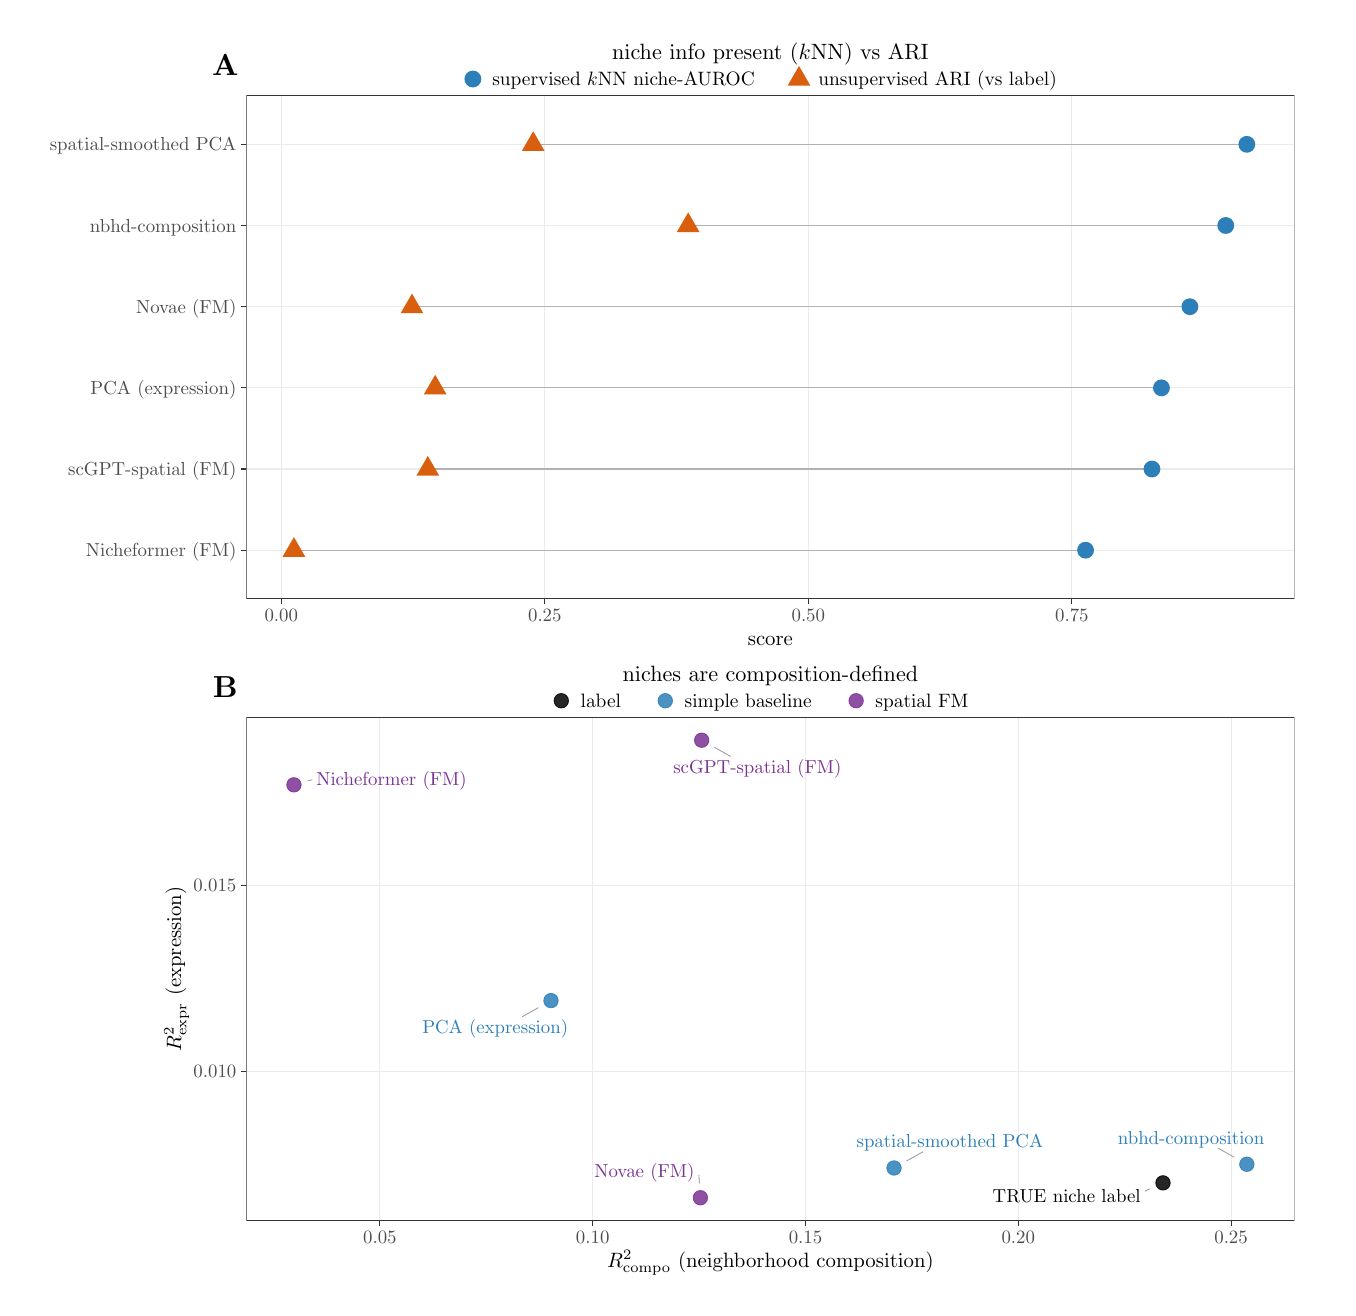
\begin{tikzpicture}[x=1pt,y=1pt]
\definecolor{fillColor}{RGB}{255,255,255}
\path[use as bounding box,fill=fillColor,fill opacity=0.00] (0,0) rectangle (469.75,455.30);
\begin{scope}
\path[clip] (  0.00,  0.00) rectangle (469.75,455.30);
\definecolor{drawColor}{RGB}{255,255,255}
\definecolor{fillColor}{RGB}{255,255,255}

\path[draw=drawColor,line width= 0.4pt,line join=round,line cap=round,fill=fillColor] ( -0.00,  0.00) rectangle (469.76,455.30);
\end{scope}
\begin{scope}
\path[clip] (  4.00,227.65) rectangle (463.75,452.30);
\definecolor{drawColor}{RGB}{255,255,255}
\definecolor{fillColor}{RGB}{255,255,255}

\path[draw=drawColor,line width= 0.4pt,line join=round,line cap=round,fill=fillColor] (  4.00,227.65) rectangle (463.75,452.30);
\end{scope}
\begin{scope}
\path[clip] (  4.00,  3.00) rectangle (463.75,227.65);
\definecolor{drawColor}{RGB}{255,255,255}
\definecolor{fillColor}{RGB}{255,255,255}

\path[draw=drawColor,line width= 0.4pt,line join=round,line cap=round,fill=fillColor] (  4.00,  3.00) rectangle (463.75,227.65);
\end{scope}
\begin{scope}
\path[clip] ( 79.00,248.88) rectangle (457.75,430.74);
\definecolor{fillColor}{RGB}{255,255,255}

\path[fill=fillColor] ( 79.00,248.88) rectangle (457.75,430.74);
\definecolor{drawColor}{gray}{0.92}

\path[draw=drawColor,line width= 0.4pt,line join=round] ( 79.00,266.48) --
	(457.75,266.48);

\path[draw=drawColor,line width= 0.4pt,line join=round] ( 79.00,295.81) --
	(457.75,295.81);

\path[draw=drawColor,line width= 0.4pt,line join=round] ( 79.00,325.14) --
	(457.75,325.14);

\path[draw=drawColor,line width= 0.4pt,line join=round] ( 79.00,354.47) --
	(457.75,354.47);

\path[draw=drawColor,line width= 0.4pt,line join=round] ( 79.00,383.81) --
	(457.75,383.81);

\path[draw=drawColor,line width= 0.4pt,line join=round] ( 79.00,413.14) --
	(457.75,413.14);

\path[draw=drawColor,line width= 0.4pt,line join=round] ( 91.64,248.88) --
	( 91.64,430.74);

\path[draw=drawColor,line width= 0.4pt,line join=round] (186.87,248.88) --
	(186.87,430.74);

\path[draw=drawColor,line width= 0.4pt,line join=round] (282.09,248.88) --
	(282.09,430.74);

\path[draw=drawColor,line width= 0.4pt,line join=round] (377.31,248.88) --
	(377.31,430.74);
\definecolor{drawColor}{gray}{0.70}

\path[draw=drawColor,line width= 0.4pt,line join=round] ( 96.21,266.48) --
	(382.26,266.48);

\path[draw=drawColor,line width= 0.4pt,line join=round] (144.59,295.81) --
	(406.26,295.81);

\path[draw=drawColor,line width= 0.4pt,line join=round] (147.25,325.14) --
	(409.69,325.14);

\path[draw=drawColor,line width= 0.4pt,line join=round] (138.87,354.47) --
	(419.97,354.47);

\path[draw=drawColor,line width= 0.4pt,line join=round] (238.67,383.81) --
	(432.92,383.81);

\path[draw=drawColor,line width= 0.4pt,line join=round] (182.68,413.14) --
	(440.54,413.14);
\definecolor{fillColor}{RGB}{217,95,14}

\path[fill=fillColor] (238.67,388.54) --
	(242.77,381.44) --
	(234.57,381.44) --
	cycle;

\path[fill=fillColor] (147.25,329.87) --
	(151.35,322.78) --
	(143.15,322.78) --
	cycle;

\path[fill=fillColor] (182.68,417.87) --
	(186.77,410.77) --
	(178.58,410.77) --
	cycle;

\path[fill=fillColor] ( 96.21,271.21) --
	(100.31,264.11) --
	( 92.11,264.11) --
	cycle;

\path[fill=fillColor] (138.87,359.21) --
	(142.97,352.11) --
	(134.77,352.11) --
	cycle;

\path[fill=fillColor] (144.59,300.54) --
	(148.69,293.44) --
	(140.49,293.44) --
	cycle;
\definecolor{fillColor}{RGB}{44,127,184}

\path[fill=fillColor] (432.92,383.81) circle (  3.04);

\path[fill=fillColor] (409.69,325.14) circle (  3.04);

\path[fill=fillColor] (440.54,413.14) circle (  3.04);

\path[fill=fillColor] (382.26,266.48) circle (  3.04);

\path[fill=fillColor] (419.97,354.47) circle (  3.04);

\path[fill=fillColor] (406.26,295.81) circle (  3.04);
\definecolor{drawColor}{gray}{0.20}

\path[draw=drawColor,line width= 0.4pt,line join=round,line cap=round] ( 79.00,248.88) rectangle (457.75,430.74);
\end{scope}
\begin{scope}
\path[clip] (  0.00,  0.00) rectangle (469.75,455.30);
\definecolor{drawColor}{gray}{0.30}

\node[text=drawColor,anchor=base east,inner sep=0pt, outer sep=0pt, scale=  0.68] at ( 75.40,264.14) {Nicheformer (FM)};

\node[text=drawColor,anchor=base east,inner sep=0pt, outer sep=0pt, scale=  0.68] at ( 75.40,293.47) {scGPT-spatial (FM)};

\node[text=drawColor,anchor=base east,inner sep=0pt, outer sep=0pt, scale=  0.68] at ( 75.40,322.80) {PCA (expression)};

\node[text=drawColor,anchor=base east,inner sep=0pt, outer sep=0pt, scale=  0.68] at ( 75.40,352.13) {Novae (FM)};

\node[text=drawColor,anchor=base east,inner sep=0pt, outer sep=0pt, scale=  0.68] at ( 75.40,381.46) {nbhd-composition};

\node[text=drawColor,anchor=base east,inner sep=0pt, outer sep=0pt, scale=  0.68] at ( 75.40,410.80) {spatial-smoothed PCA};
\end{scope}
\begin{scope}
\path[clip] (  0.00,  0.00) rectangle (469.75,455.30);
\definecolor{drawColor}{gray}{0.20}

\path[draw=drawColor,line width= 0.4pt,line join=round] ( 77.00,266.48) --
	( 79.00,266.48);

\path[draw=drawColor,line width= 0.4pt,line join=round] ( 77.00,295.81) --
	( 79.00,295.81);

\path[draw=drawColor,line width= 0.4pt,line join=round] ( 77.00,325.14) --
	( 79.00,325.14);

\path[draw=drawColor,line width= 0.4pt,line join=round] ( 77.00,354.47) --
	( 79.00,354.47);

\path[draw=drawColor,line width= 0.4pt,line join=round] ( 77.00,383.81) --
	( 79.00,383.81);

\path[draw=drawColor,line width= 0.4pt,line join=round] ( 77.00,413.14) --
	( 79.00,413.14);
\end{scope}
\begin{scope}
\path[clip] (  0.00,  0.00) rectangle (469.75,455.30);
\definecolor{drawColor}{gray}{0.20}

\path[draw=drawColor,line width= 0.4pt,line join=round] ( 91.64,246.88) --
	( 91.64,248.88);

\path[draw=drawColor,line width= 0.4pt,line join=round] (186.87,246.88) --
	(186.87,248.88);

\path[draw=drawColor,line width= 0.4pt,line join=round] (282.09,246.88) --
	(282.09,248.88);

\path[draw=drawColor,line width= 0.4pt,line join=round] (377.31,246.88) --
	(377.31,248.88);
\end{scope}
\begin{scope}
\path[clip] (  0.00,  0.00) rectangle (469.75,455.30);
\definecolor{drawColor}{gray}{0.30}

\node[text=drawColor,anchor=base,inner sep=0pt, outer sep=0pt, scale=  0.68] at ( 91.64,240.60) {0.00};

\node[text=drawColor,anchor=base,inner sep=0pt, outer sep=0pt, scale=  0.68] at (186.87,240.60) {0.25};

\node[text=drawColor,anchor=base,inner sep=0pt, outer sep=0pt, scale=  0.68] at (282.09,240.60) {0.50};

\node[text=drawColor,anchor=base,inner sep=0pt, outer sep=0pt, scale=  0.68] at (377.31,240.60) {0.75};
\end{scope}
\begin{scope}
\path[clip] (  0.00,  0.00) rectangle (469.75,455.30);
\definecolor{drawColor}{RGB}{0,0,0}

\node[text=drawColor,anchor=base,inner sep=0pt, outer sep=0pt, scale=  0.75] at (268.38,232.11) {score};
\end{scope}
\begin{scope}
\path[clip] (  0.00,  0.00) rectangle (469.75,455.30);
\definecolor{fillColor}{RGB}{255,255,255}

\path[fill=fillColor] (155.88,432.74) rectangle (380.88,440.74);
\end{scope}
\begin{scope}
\path[clip] (  0.00,  0.00) rectangle (469.75,455.30);
\definecolor{fillColor}{RGB}{255,255,255}

\path[fill=fillColor] (156.88,432.74) rectangle (164.88,440.74);
\definecolor{fillColor}{RGB}{44,127,184}

\path[fill=fillColor] (160.88,436.74) circle (  3.04);
\end{scope}
\begin{scope}
\path[clip] (  0.00,  0.00) rectangle (469.75,455.30);
\definecolor{fillColor}{RGB}{255,255,255}

\path[fill=fillColor] (274.72,432.74) rectangle (282.72,440.74);
\definecolor{fillColor}{RGB}{217,95,14}

\path[fill=fillColor] (278.72,441.47) --
	(282.82,434.37) --
	(274.62,434.37) --
	cycle;
\end{scope}
\begin{scope}
\path[clip] (  0.00,  0.00) rectangle (469.75,455.30);
\definecolor{drawColor}{RGB}{0,0,0}

\node[text=drawColor,anchor=base west,inner sep=0pt, outer sep=0pt, scale=  0.70] at (167.88,434.33) {supervised $k$NN niche-AUROC};
\end{scope}
\begin{scope}
\path[clip] (  0.00,  0.00) rectangle (469.75,455.30);
\definecolor{drawColor}{RGB}{0,0,0}

\node[text=drawColor,anchor=base west,inner sep=0pt, outer sep=0pt, scale=  0.70] at (285.72,434.33) {unsupervised ARI (vs label)};
\end{scope}
\begin{scope}
\path[clip] (  0.00,  0.00) rectangle (469.75,455.30);
\definecolor{drawColor}{RGB}{0,0,0}

\node[text=drawColor,anchor=base,inner sep=0pt, outer sep=0pt, scale=  0.80] at (268.38,443.79) {niche info present ($k$NN) vs ARI};
\end{scope}
\begin{scope}
\path[clip] (  0.00,  0.00) rectangle (469.75,455.30);
\definecolor{drawColor}{RGB}{0,0,0}

\node[text=drawColor,anchor=base,inner sep=0pt, outer sep=0pt, scale=  1.10] at ( 71.42,437.85) {\bfseries A};
\end{scope}
\begin{scope}
\path[clip] ( 79.00, 24.23) rectangle (457.75,206.09);
\definecolor{fillColor}{RGB}{255,255,255}

\path[fill=fillColor] ( 79.00, 24.23) rectangle (457.75,206.09);
\definecolor{drawColor}{gray}{0.92}

\path[draw=drawColor,line width= 0.4pt,line join=round] ( 79.00, 78.19) --
	(457.75, 78.19);

\path[draw=drawColor,line width= 0.4pt,line join=round] ( 79.00,145.40) --
	(457.75,145.40);

\path[draw=drawColor,line width= 0.4pt,line join=round] (127.28, 24.23) --
	(127.28,206.09);

\path[draw=drawColor,line width= 0.4pt,line join=round] (204.17, 24.23) --
	(204.17,206.09);

\path[draw=drawColor,line width= 0.4pt,line join=round] (281.06, 24.23) --
	(281.06,206.09);

\path[draw=drawColor,line width= 0.4pt,line join=round] (357.96, 24.23) --
	(357.96,206.09);

\path[draw=drawColor,line width= 0.4pt,line join=round] (434.85, 24.23) --
	(434.85,206.09);
\definecolor{drawColor}{RGB}{0,0,0}
\definecolor{fillColor}{RGB}{0,0,0}

\path[draw=drawColor,draw opacity=0.85,line width= 0.3pt,line join=round,line cap=round,fill=fillColor,fill opacity=0.85] (410.24, 37.87) circle (  2.61);
\definecolor{drawColor}{RGB}{44,127,184}
\definecolor{fillColor}{RGB}{44,127,184}

\path[draw=drawColor,draw opacity=0.85,line width= 0.3pt,line join=round,line cap=round,fill=fillColor,fill opacity=0.85] (440.54, 44.59) circle (  2.61);

\path[draw=drawColor,draw opacity=0.85,line width= 0.3pt,line join=round,line cap=round,fill=fillColor,fill opacity=0.85] (189.10,103.73) circle (  2.61);

\path[draw=drawColor,draw opacity=0.85,line width= 0.3pt,line join=round,line cap=round,fill=fillColor,fill opacity=0.85] (313.05, 43.25) circle (  2.61);
\definecolor{drawColor}{RGB}{123,50,148}
\definecolor{fillColor}{RGB}{123,50,148}

\path[draw=drawColor,draw opacity=0.85,line width= 0.3pt,line join=round,line cap=round,fill=fillColor,fill opacity=0.85] ( 96.21,181.69) circle (  2.61);

\path[draw=drawColor,draw opacity=0.85,line width= 0.3pt,line join=round,line cap=round,fill=fillColor,fill opacity=0.85] (243.08, 32.49) circle (  2.61);

\path[draw=drawColor,draw opacity=0.85,line width= 0.3pt,line join=round,line cap=round,fill=fillColor,fill opacity=0.85] (243.54,197.82) circle (  2.61);
\definecolor{drawColor}{gray}{0.60}

\path[draw=drawColor,line width= 0.3pt,line join=round,line cap=round] (403.77, 34.87) -- (405.45, 35.65);

\path[draw=drawColor,line width= 0.3pt,line join=round,line cap=round] (430.18, 50.39) -- (435.93, 47.17);

\path[draw=drawColor,line width= 0.3pt,line join=round,line cap=round] (178.70, 97.90) -- (184.49,101.15);

\path[draw=drawColor,line width= 0.3pt,line join=round,line cap=round] (323.46, 49.08) -- (317.66, 45.83);

\path[draw=drawColor,line width= 0.3pt,line join=round,line cap=round] (102.71,183.52) -- (101.30,183.13);

\path[draw=drawColor,line width= 0.3pt,line join=round,line cap=round] (242.54, 40.67) -- (242.73, 37.77);

\path[draw=drawColor,line width= 0.3pt,line join=round,line cap=round] (253.90,192.02) -- (248.15,195.24);
\definecolor{drawColor}{RGB}{0,0,0}

\node[text=drawColor,anchor=base,inner sep=0pt, outer sep=0pt, scale=  0.68] at (375.43, 30.87) {TRUE niche label};
\definecolor{drawColor}{RGB}{44,127,184}

\node[text=drawColor,anchor=base,inner sep=0pt, outer sep=0pt, scale=  0.68] at (420.41, 51.90) {nbhd-composition};

\node[text=drawColor,anchor=base,inner sep=0pt, outer sep=0pt, scale=  0.68] at (168.93, 91.70) {PCA (expression)};

\node[text=drawColor,anchor=base,inner sep=0pt, outer sep=0pt, scale=  0.68] at (333.24, 50.59) {spatial-smoothed PCA};
\definecolor{drawColor}{RGB}{123,50,148}

\node[text=drawColor,anchor=base,inner sep=0pt, outer sep=0pt, scale=  0.68] at (131.50,181.60) {Nicheformer (FM)};

\node[text=drawColor,anchor=base,inner sep=0pt, outer sep=0pt, scale=  0.68] at (222.87, 39.85) {Novae (FM)};

\node[text=drawColor,anchor=base,inner sep=0pt, outer sep=0pt, scale=  0.68] at (263.68,185.81) {scGPT-spatial (FM)};
\definecolor{drawColor}{gray}{0.20}

\path[draw=drawColor,line width= 0.4pt,line join=round,line cap=round] ( 79.00, 24.23) rectangle (457.75,206.09);
\end{scope}
\begin{scope}
\path[clip] (  0.00,  0.00) rectangle (469.75,455.30);
\definecolor{drawColor}{gray}{0.20}

\path[draw=drawColor,line width= 0.4pt,line join=round] (127.28, 22.23) --
	(127.28, 24.23);

\path[draw=drawColor,line width= 0.4pt,line join=round] (204.17, 22.23) --
	(204.17, 24.23);

\path[draw=drawColor,line width= 0.4pt,line join=round] (281.06, 22.23) --
	(281.06, 24.23);

\path[draw=drawColor,line width= 0.4pt,line join=round] (357.96, 22.23) --
	(357.96, 24.23);

\path[draw=drawColor,line width= 0.4pt,line join=round] (434.85, 22.23) --
	(434.85, 24.23);
\end{scope}
\begin{scope}
\path[clip] (  0.00,  0.00) rectangle (469.75,455.30);
\definecolor{drawColor}{gray}{0.30}

\node[text=drawColor,anchor=base,inner sep=0pt, outer sep=0pt, scale=  0.68] at (127.28, 15.95) {0.05};

\node[text=drawColor,anchor=base,inner sep=0pt, outer sep=0pt, scale=  0.68] at (204.17, 15.95) {0.10};

\node[text=drawColor,anchor=base,inner sep=0pt, outer sep=0pt, scale=  0.68] at (281.06, 15.95) {0.15};

\node[text=drawColor,anchor=base,inner sep=0pt, outer sep=0pt, scale=  0.68] at (357.96, 15.95) {0.20};

\node[text=drawColor,anchor=base,inner sep=0pt, outer sep=0pt, scale=  0.68] at (434.85, 15.95) {0.25};
\end{scope}
\begin{scope}
\path[clip] (  0.00,  0.00) rectangle (469.75,455.30);
\definecolor{drawColor}{RGB}{0,0,0}

\node[text=drawColor,anchor=base,inner sep=0pt, outer sep=0pt, scale=  0.75] at (268.38,  7.46) {$R^2_{\mathrm{compo}}$ (neighborhood composition)};
\end{scope}
\begin{scope}
\path[clip] (  0.00,  0.00) rectangle (469.75,455.30);
\definecolor{drawColor}{gray}{0.30}

\node[text=drawColor,anchor=base east,inner sep=0pt, outer sep=0pt, scale=  0.68] at ( 75.40, 75.85) {0.010};

\node[text=drawColor,anchor=base east,inner sep=0pt, outer sep=0pt, scale=  0.68] at ( 75.40,143.06) {0.015};
\end{scope}
\begin{scope}
\path[clip] (  0.00,  0.00) rectangle (469.75,455.30);
\definecolor{drawColor}{gray}{0.20}

\path[draw=drawColor,line width= 0.4pt,line join=round] ( 77.00, 78.19) --
	( 79.00, 78.19);

\path[draw=drawColor,line width= 0.4pt,line join=round] ( 77.00,145.40) --
	( 79.00,145.40);
\end{scope}
\begin{scope}
\path[clip] (  0.00,  0.00) rectangle (469.75,455.30);
\definecolor{drawColor}{RGB}{0,0,0}

\node[text=drawColor,rotate= 90.00,anchor=base,inner sep=0pt, outer sep=0pt, scale=  0.75] at ( 55.45,115.16) {$R^2_{\mathrm{expr}}$ (expression)};
\end{scope}
\begin{scope}
\path[clip] (  0.00,  0.00) rectangle (469.75,455.30);
\definecolor{fillColor}{RGB}{255,255,255}

\path[fill=fillColor] (187.82,208.09) rectangle (348.93,216.09);
\end{scope}
\begin{scope}
\path[clip] (  0.00,  0.00) rectangle (469.75,455.30);
\definecolor{fillColor}{RGB}{255,255,255}

\path[fill=fillColor] (188.82,208.09) rectangle (196.82,216.09);
\definecolor{drawColor}{RGB}{0,0,0}
\definecolor{fillColor}{RGB}{0,0,0}

\path[draw=drawColor,draw opacity=0.85,line width= 0.3pt,line join=round,line cap=round,fill=fillColor,fill opacity=0.85] (192.82,212.09) circle (  2.61);
\end{scope}
\begin{scope}
\path[clip] (  0.00,  0.00) rectangle (469.75,455.30);
\definecolor{fillColor}{RGB}{255,255,255}

\path[fill=fillColor] (226.40,208.09) rectangle (234.40,216.09);
\definecolor{drawColor}{RGB}{44,127,184}
\definecolor{fillColor}{RGB}{44,127,184}

\path[draw=drawColor,draw opacity=0.85,line width= 0.3pt,line join=round,line cap=round,fill=fillColor,fill opacity=0.85] (230.40,212.09) circle (  2.61);
\end{scope}
\begin{scope}
\path[clip] (  0.00,  0.00) rectangle (469.75,455.30);
\definecolor{fillColor}{RGB}{255,255,255}

\path[fill=fillColor] (295.36,208.09) rectangle (303.36,216.09);
\definecolor{drawColor}{RGB}{123,50,148}
\definecolor{fillColor}{RGB}{123,50,148}

\path[draw=drawColor,draw opacity=0.85,line width= 0.3pt,line join=round,line cap=round,fill=fillColor,fill opacity=0.85] (299.36,212.09) circle (  2.61);
\end{scope}
\begin{scope}
\path[clip] (  0.00,  0.00) rectangle (469.75,455.30);
\definecolor{drawColor}{RGB}{0,0,0}

\node[text=drawColor,anchor=base west,inner sep=0pt, outer sep=0pt, scale=  0.70] at (199.82,209.68) {label};
\end{scope}
\begin{scope}
\path[clip] (  0.00,  0.00) rectangle (469.75,455.30);
\definecolor{drawColor}{RGB}{0,0,0}

\node[text=drawColor,anchor=base west,inner sep=0pt, outer sep=0pt, scale=  0.70] at (237.40,209.68) {simple baseline};
\end{scope}
\begin{scope}
\path[clip] (  0.00,  0.00) rectangle (469.75,455.30);
\definecolor{drawColor}{RGB}{0,0,0}

\node[text=drawColor,anchor=base west,inner sep=0pt, outer sep=0pt, scale=  0.70] at (306.36,209.68) {spatial FM};
\end{scope}
\begin{scope}
\path[clip] (  0.00,  0.00) rectangle (469.75,455.30);
\definecolor{drawColor}{RGB}{0,0,0}

\node[text=drawColor,anchor=base,inner sep=0pt, outer sep=0pt, scale=  0.80] at (268.38,219.14) {niches are composition-defined};
\end{scope}
\begin{scope}
\path[clip] (  0.00,  0.00) rectangle (469.75,455.30);
\definecolor{drawColor}{RGB}{0,0,0}

\node[text=drawColor,anchor=base,inner sep=0pt, outer sep=0pt, scale=  1.10] at ( 71.42,213.20) {\bfseries B};
\end{scope}
\end{tikzpicture}
